\documentclass[12pt]{ximera}
\title{Final Exam}
\begin{document}
\begin{abstract}
The cumulative final: zero-sum games and saddle points, a two-set Venn diagram,
counting with restrictions, the subtraction game, a modified Rock/Paper/Scissors, and
a mixed-strategy equilibrium, plus bonus problems from across the semester.
\end{abstract}
\maketitle

\section*{Final Exam}

\begin{problem}
Assess whether each of the following claims is true or false.

\begin{prompt}
\textbf{(a)} Claim: a zero-sum game is a game where every point earned by one of the
players is lost by the other.

\begin{multipleChoice}
\choice[correct]{True}
\choice{False}
\end{multipleChoice}

\begin{feedback}
True --- that is the definition of zero-sum: the players' payoffs always add to zero.
\end{feedback}
\end{prompt}

\begin{prompt}
\textbf{(b)} Claim: if a two-player zero-sum game has a saddle point, then the expected
value of the game is the value of that saddle point.

\begin{multipleChoice}
\choice[correct]{True}
\choice{False}
\end{multipleChoice}

\begin{feedback}
True. At a saddle point neither player gains by switching strategies, so optimal play
settles there every time, and the game is worth exactly that entry. Playing any other
strategy only lets the opponent do better.
\end{feedback}
\end{prompt}
\end{problem}

\begin{problem}
In a survey of $250$ people, $87$ of the participants said they agree that cereal is
a kind of soup (CS), $103$ said they agree that poptarts are a kind of ravioli (PR),
and $58$ said they agree with both.

\begin{prompt}
\textbf{(a)} Fill in all four regions of the Venn diagram.

\begin{center}
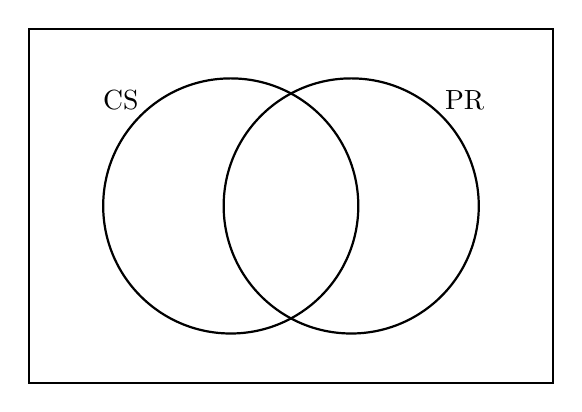
\begin{tikzpicture}[scale=0.9]
  \draw[thick] (-0.85,0) circle (1.8) node at (-2.4,1.5) {CS};
  \draw[thick] (0.85,0) circle (1.8) node at (2.45,1.5) {PR};
  \draw[thick] (-3.7,-2.5) rectangle (3.7,2.5);
\end{tikzpicture}
\end{center}

CS only: $\answer{29}$ \qquad
Both: $\answer{58}$ \qquad
PR only: $\answer{45}$ \qquad
Neither: $\answer{118}$

\begin{hint}
The $87$ and $103$ each already include the $58$ who agreed with both.
\end{hint}

\begin{feedback}
The overlap is $58$. Peeling it off each circle:
\[
\text{CS only} = 87-58 = 29, \qquad \text{PR only} = 103-58 = 45.
\]
Those three regions total $29+58+45=132$, so the region outside both circles is
\[ 250-132 = 118. \]
\end{feedback}
\end{prompt}

\begin{prompt}
\textbf{(b)} What is the (conditional) probability that someone who agrees that cereal
is a kind of soup does NOT agree that poptarts are a kind of ravioli?

Give your answer as a fraction in lowest terms: $\answer{1/3}$

\begin{feedback}
Restrict to the $87$ people who agree cereal is soup. Of those, $29$ are in the ``CS
only'' region, meaning they do not agree about poptarts. So
\[
P\!\left(\olsi{PR}\mid CS\right)=\frac{29}{87}=\frac13.
\]
\end{feedback}
\end{prompt}
\end{problem}

\begin{problem}
It's nearly girl scout cookie season, and an office manager needs to choose which six
of the eleven varieties of girl scout cookies currently available to buy for the office.

\begin{prompt}
\textbf{(a)} How many different sets of six could possibly be selected from among the
eleven available cookie varieties?

$\answer{462}$

\begin{feedback}
\[ C(11,6)=\frac{11!}{6!\,5!}=462. \]
\end{feedback}
\end{prompt}

\begin{prompt}
\textbf{(b)} Two of the eleven available varieties are gluten-free. If the manager
wants \emph{exactly one} of the chosen cookie varieties to be gluten-free, how many
different sets of six are possible?

$\answer{252}$

\begin{hint}
Split the decision in two: which gluten-free variety, and which of the others fill
the remaining five slots.
\end{hint}

\begin{feedback}
Choose $1$ of the $2$ gluten-free varieties, and then $5$ of the $9$ remaining
varieties:
\[
C(2,1)\cdot C(9,5) = 2\cdot 126 = 252.
\]
\end{feedback}
\end{prompt}

\begin{prompt}
\textbf{(c)} How many different sets of six don't include \emph{any} gluten-free
varieties?

$\answer{84}$

\begin{feedback}
All six must come from the $9$ varieties that are not gluten-free:
\[ C(9,6)=\frac{9!}{6!\,3!}=84. \]
\end{feedback}
\end{prompt}

\begin{prompt}
\textbf{(d)} If the manager chooses six at random from among the eleven available cookie
varieties, what is the probability that \emph{at least one} of the varieties I select
is gluten-free?

Give your answer as a fraction in lowest terms: $\answer{9/11}$

\begin{feedback}
Use the complement with part (c):
\[
P(\text{no gluten-free}) = \frac{84}{462} = \frac{2}{11},
\]
so
\[
P(\text{at least one}) = 1-\frac{2}{11} = \frac{9}{11}\approx 0.818,
\]
about $81.8\%$.
\end{feedback}
\end{prompt}
\end{problem}

\begin{problem}
Alice and Bob are playing a variation of the Subtraction Game with the following
rules:
\begin{itemize}
\item start with $18$ stones in the pile;
\item on each turn, a player can take $1$, $2$, or $3$ stones;
\item the winner is the player who takes the final stone.
\end{itemize}

\begin{prompt}
If Alice goes first, which player has a winning strategy?

\begin{multipleChoice}
\choice[correct]{Alice, the first player}
\choice{Bob, the second player}
\choice{Neither --- it depends on how Bob plays}
\end{multipleChoice}

\begin{hint}
Work backwards. Which pile sizes are losing positions for the player whose turn it
is? Start with $4$.
\end{hint}

\begin{feedback}
Alice has the winning strategy.

The losing positions --- the pile sizes you do \emph{not} want to face on your turn ---
are the multiples of $4$. If you face $4$ stones, whatever you take ($1$, $2$, or
$3$), your opponent can take the rest and win. If you face $8$, any move leaves
between $5$ and $7$, from which your opponent can move back down to exactly $4$, and
so on.

Since $18$ is not a multiple of $4$ ($18 = 4\cdot 4 + 2$), the first player wins.
\end{feedback}
\end{prompt}

\begin{prompt}
What is that winning strategy? How many stones should Alice take on her first turn?

$\answer{2}$ stones.

\begin{feedback}
Alice takes $2$ stones, leaving $16$ --- a multiple of $4$ --- for Bob.

From then on, she answers each of Bob's moves so that the two moves together remove
exactly $4$ stones: if Bob takes $1$, she takes $3$; if Bob takes $2$, she takes $2$;
if Bob takes $3$, she takes $1$. Each round drops the pile by $4$, so Bob faces
$16, 12, 8, 4$ in turn, and finally $0$ --- meaning Alice took the last stone.
\end{feedback}
\end{prompt}
\end{problem}

\begin{problem}
The following payoff matrices each represent Alice's perspective for a zero-sum game.
Identify the saddle point if it exists.

\begin{prompt}
\textbf{(a)}
\[
\begin{array}{c|c|c|}
\phantom{|} & c & d \\\hline
a & -7 & 2 \\\hline
b & 0 & 5 \\\hline
\end{array}
\]
Does a saddle point exist?
\begin{multipleChoice}
\choice[correct]{Yes}
\choice{No}
\end{multipleChoice}
If so, its value is $\answer{0}$.

\begin{feedback}
Row minima $-7$ and $0$ give a maximin of $0$; column maxima $0$ and $5$ give a minimax
of $0$. The saddle point is $0$ at cell $(b,c)$.
\end{feedback}
\end{prompt}

\begin{prompt}
\textbf{(b)}
\[
\begin{array}{c|c|c|}
\phantom{|} & c & d \\\hline
a & 4 & -3 \\\hline
b & -1 & 2 \\\hline
\end{array}
\]
Does a saddle point exist?
\begin{multipleChoice}
\choice{Yes}
\choice[correct]{No}
\end{multipleChoice}

\begin{feedback}
Row minima $-3$ and $-1$ give a maximin of $-1$; column maxima $4$ and $2$ give a minimax
of $2$. Since $-1 \neq 2$, there is no saddle point, so neither player has a stable pure
strategy.
\end{feedback}
\end{prompt}

\begin{prompt}
\textbf{(c)}
\[
\begin{array}{c|c|c|c|}
\phantom{|} & d & e & f \\\hline
a & -1 & 5 & 0 \\\hline
b & -2 & 0 & -3 \\\hline
c & 2 & 3 & 1 \\\hline
\end{array}
\]
Does a saddle point exist?
\begin{multipleChoice}
\choice[correct]{Yes}
\choice{No}
\end{multipleChoice}
If so, its value is $\answer{1}$.

\begin{feedback}
Row minima are $-1$, $-3$, and $1$, so the maximin is $1$. Column maxima are $2$, $5$,
and $1$, so the minimax is $1$. The saddle point is $1$ at cell $(c,f)$.
\end{feedback}
\end{prompt}

\begin{prompt}
\textbf{(d)}
\[
\begin{array}{c|c|c|}
\phantom{|} & d & e \\\hline
a & 0 & -3 \\\hline
b & 2 & 4 \\\hline
c & -5 & 1 \\\hline
\end{array}
\]
Does a saddle point exist?
\begin{multipleChoice}
\choice[correct]{Yes}
\choice{No}
\end{multipleChoice}
If so, its value is $\answer{2}$.

\begin{feedback}
Row minima are $-3$, $2$, and $-5$, so the maximin is $2$. Column maxima are $2$ and $4$,
so the minimax is $2$. The saddle point is $2$ at cell $(b,d)$.

Row $b$ dominates both other rows for Alice, and column $d$ dominates $e$ for Bob, so
both players' choices are forced.
\end{feedback}
\end{prompt}
\end{problem}

\begin{problem}
Complete the payoff matrix from Alice's perspective for a two-player zero-sum game
similar to Rock/Paper/Scissors, except that only Alice has paper and only Bob has
scissors:
\begin{itemize}
\item rock wins \emph{1 point} versus scissors;
\item scissors wins \emph{2 points} versus paper;
\item paper wins \emph{1 point} versus rock;
\item everything else is a tie.
\end{itemize}

\[
\begin{array}{c|c|c|}
\phantom{|} & \text{Bob: rock} & \text{Bob: scissors} \\\hline
\text{Alice: rock} & \answer{0} & \answer{1} \\\hline
\text{Alice: paper} & \answer{1} & \answer{-2} \\\hline
\end{array}
\]

\begin{hint}
Entries are from Alice's perspective, so a win for Bob is negative.
\end{hint}

\begin{feedback}
\begin{itemize}
\item rock vs.\ rock: a tie, $0$.
\item rock vs.\ scissors: rock wins $1$ point for Alice, $+1$.
\item paper vs.\ rock: paper wins $1$ point for Alice, $+1$.
\item paper vs.\ scissors: scissors wins $2$ points for Bob, $-2$.
\end{itemize}

This game has no saddle point: the maximin is $-2$ and the minimax is $1$.
\end{feedback}
\end{problem}

\begin{problem}
Suppose the following payoff matrix represents Alice's perspective for a zero-sum game.
\[
\begin{array}{c|c|c|}
\phantom{|} & \text{Bob: }a & \text{Bob: }b \\\hline
\text{Alice: }a & 1 & 4 \\\hline
\text{Alice: }b & 3 & 0 \\\hline
\end{array}
\]

\begin{prompt}
\textbf{(a)} Determine Bob's stable mixed strategy at the \emph{equilibrium point} of
this game. Enter fractions.

$P(\text{Bob plays } a)=\answer{2/3}$ \qquad $P(\text{Bob plays } b)=\answer{1/3}$

\begin{hint}
Let Bob play $a$ with probability $q$. Choose $q$ so that Alice's two strategies have
equal expected value.
\end{hint}

\begin{feedback}
There is no saddle point: the maximin is $1$ and the minimax is $3$.

With Bob playing $a$ with probability $q$, Alice's expected payoffs are
\[
\text{row } a:\ 1q+4(1-q)=4-3q, \qquad \text{row } b:\ 3q+0(1-q)=3q.
\]
Setting them equal, $4-3q=3q$, so $q=\frac23$. Bob plays $a$ two-thirds of the time
and $b$ one-third.
\end{feedback}
\end{prompt}

\begin{prompt}
\textbf{(b)} Alice's stable mixed strategy is to play $a$ and $b$ with probability
$50\%$ each. Using this and Bob's strategy from part (a), calculate the expected value
of the game.

$\answer[tolerance=0.001]{2}$

\begin{feedback}
The four cells occur with probabilities
\[
P(a,a)=\tfrac12\cdot\tfrac23=\tfrac13,\quad P(a,b)=\tfrac12\cdot\tfrac13=\tfrac16,\quad
P(b,a)=\tfrac13,\quad P(b,b)=\tfrac16,
\]
so
\[
E=1\cdot\tfrac13+4\cdot\tfrac16+3\cdot\tfrac13+0\cdot\tfrac16=\tfrac13+\tfrac23+1=2.
\]
Check: Alice's $50\%$ mix does make Bob indifferent --- column $a$ gives
$\frac12(1)+\frac12(3)=2$ and column $b$ gives $\frac12(4)+\frac12(0)=2$.
\end{feedback}
\end{prompt}
\end{problem}

\begin{problem}
The following are bonus problems from throughout the semester.

\begin{prompt}
\textbf{(a)} Use the Principle of Inclusion-Exclusion to calculate $n(A\cap B)$ if
you know that $n(A)=25$, $n(B)=55$, and $n(A\cup B)=65$.

$\answer{15}$

\begin{feedback}
\[ 65 = 25 + 55 - n(A\cap B) = 80 - n(A\cap B), \]
so $n(A\cap B)=80-65=15$.
\end{feedback}
\end{prompt}

\begin{prompt}
\textbf{(b)} Shade the regions of a three-circle Venn diagram to show
$(A\cup B)\cap C$. Sketch it on paper, then check the solution.

\begin{freeResponse}
\end{freeResponse}

\begin{feedback}
Keep only the parts of $A$ and $B$ that also lie inside $C$.
\begin{center}
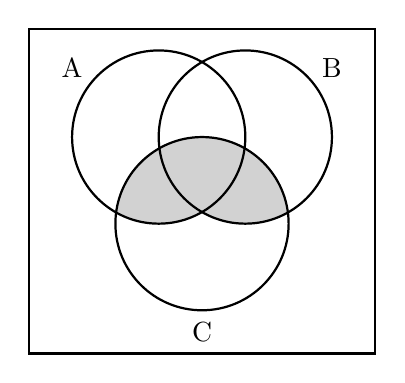
\begin{tikzpicture}[scale=1.1]
  \begin{scope}
    \clip (0.5,-1) circle (1);
    \fill[gray!35] (0,0) circle (1);
    \fill[gray!35] (1,0) circle (1);
  \end{scope}
  \draw[thick] (0,0) circle (1) node at (-1,0.8) {A};
  \draw[thick] (1,0) circle (1) node at (2,0.8) {B};
  \draw[thick] (0.5,-1) circle (1) node at (0.5,-2.25) {C};
  \draw[thick] (-1.5,-2.5) rectangle (2.5,1.25);
\end{tikzpicture}
\end{center}
\end{feedback}
\end{prompt}

\begin{prompt}
\textbf{(c)} Calculate by hand the combination $C(10,6)$.

$\answer{210}$

\begin{feedback}
\[
C(10,6)=\frac{10!}{6!\,4!}
=\frac{10\cdot 9\cdot 8\cdot 7}{4\cdot 3\cdot 2\cdot 1}
=\frac{5040}{24}=210.
\]
Note that $C(10,6)=C(10,4)$, so it is easier to cancel the larger factorial.
\end{feedback}
\end{prompt}

\begin{prompt}
\textbf{(d)} Suppose you repeat an experiment five times, and each time the
probability of success is $60\%$. Calculate the (binomial) probability that you record
exactly three successes.

As a percentage rounded to two decimal places: $\answer[tolerance=0.005]{34.56}\%$

\begin{feedback}
\[
P(X=3)=C(5,3)(0.6)^3(0.4)^2 = 10(0.216)(0.16) = 0.3456,
\]
that is, $34.56\%$.
\end{feedback}
\end{prompt}

\begin{prompt}
\textbf{(e)} Calculate the expected winnings of a raffle with the following
probability distribution:

\begin{center}
\begin{tabular}{|r|c|c|c|c|}\hline
Total winnings: & $-\$1$ & \$0 & \$5 & \$10 \\\hline
Probability of each: & $0.6$ & $0.25$ & $0.1$ & $0.05$ \\\hline
\end{tabular}
\end{center}

$\$\answer[tolerance=0.005]{0.40}$

\begin{feedback}
\begin{align*}
E(X) &= 0.6(-1) + 0.25(0) + 0.1(5) + 0.05(10)\\
     &= -0.60 + 0 + 0.50 + 0.50 = 0.40.
\end{align*}
So the expected winnings are $\$0.40$ per raffle --- a favorable game for the player,
even though the most likely single outcome is losing a dollar.
\end{feedback}
\end{prompt}
\end{problem}

\end{document}
